In this chapter, we will introduce \index{infinite impulse
response}{infinite impulse response} (\index{IIR}{IIR}) filters. Just like finite
impulse response filters (FIR), they are also linear time-invariant
systems. The main difference is that infinite impulse response filters
include feedback from the samples of the output signal $y[n]$ of the
system, and as the name already implies, this feedback makes the
impulse response of the system infinitely long.

The advantage of IIR filters compared to FIR filters is that it is
often possible to design a lower order filter, which meets design
requirements for a frequency response. The lower the order of the
filter, the fewer computations per output sample are needed. This is
important in some digital signal processing applications, especially
ones where the sampling rate of the signal is very large and there are
strict requirements for realtime processing speeds.

A drawback of IIR filters is that the feedback terms can result in an
unstable filter output. These types of filters are also often not
as accurate numerically as FIR filters.

\section{Infinite impulse response filter}
Consider the following system:
\begin{equation}
\boxed{
y[n] = \underbrace{\sum_{\ell=1}^{N} a_{\ell} y[n-\ell]}_{\mathrm{feedback~terms}} + \underbrace{\sum_{k=0}^{M} b_k x[n-k]}_{\mathrm{feed~forward~terms}}
\label{eq:iir_def}
}
\end{equation}
The filter output depends on the current and past values of the input
signal, as well as past values of the \emph{system output}
$y[n]$. This is a causal system\sidenote{a system is causal if it only depends on present and past values.}, because the system output does not
depend on future values of the input or output signal.

The system defined in Equation \ref{eq:iir_def} is called an infinite
impulse response filter. A total of $N+M+1$ filter coefficients
$a_{\ell}$ and $b_k$ are needed to specify this filter.

\section{System function}

The system function, i.e., the $z$-transform of the impulse response for an IIR filter, is:
\begin{equation}
\boxed{
\Hez = \frac{\sum_{k=0}^{M}b_k z^{-k}}{1-\sum_{\ell=1}^{N}a_\ell z^{-\ell}}
\label{eq:iir_system_gen}
}
\end{equation}

\begin{marginfigure}
\begin{center}
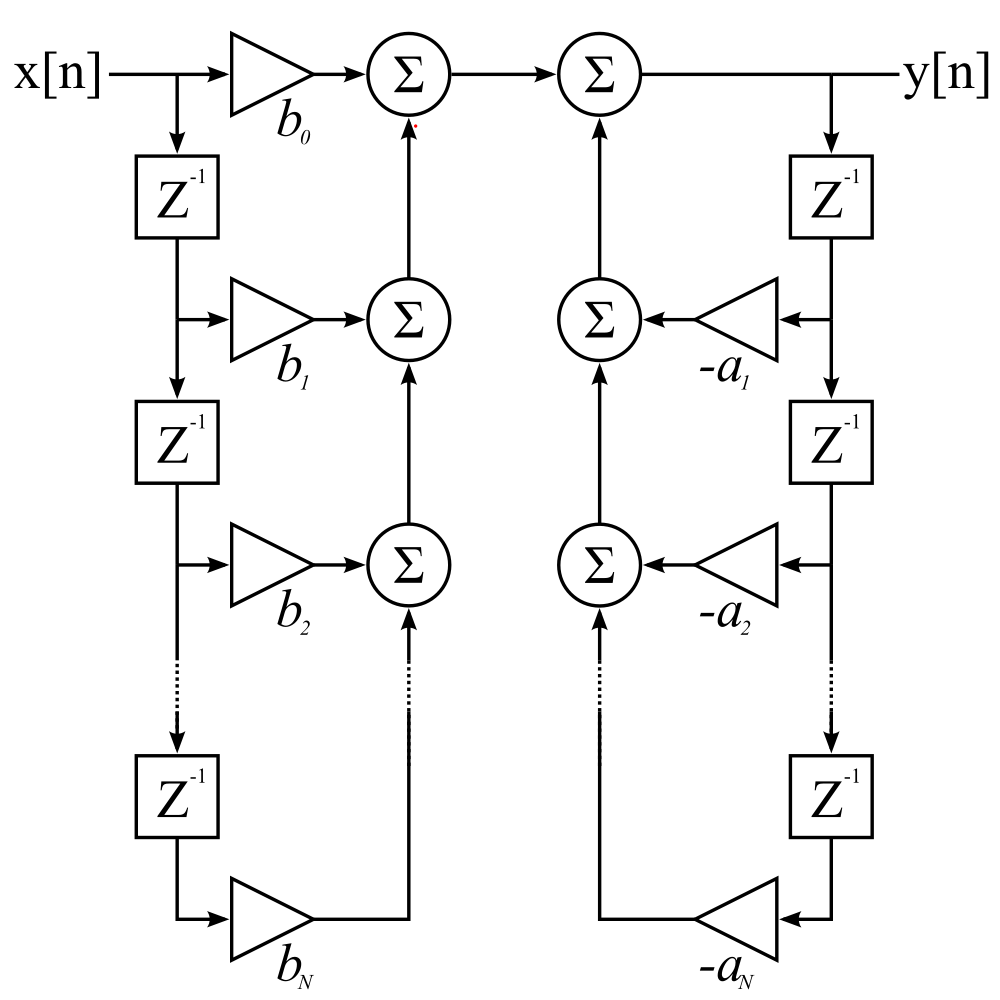
\includegraphics[width=\textwidth]{ch19/figures/iir.png}
\end{center}
\caption{A block diagram representation of an infinite impulse response filter system function.}
\label{fig:iireq}
\end{marginfigure}

\begin{proof}
Apply the $z$-transform to the definition of the IIR, and use linearity and time-shift properties:
\begin{align}
y[n] &= \left.\sum_{\ell=1}^{N} a_{\ell} y[n-\ell] + \sum_{k=0}^{M} b_k x[n-k]~~\right| \mathcal{Z}\{ \cdot \} \\
Y(z) &= \sum_{\ell = 1}^{N} a_{\ell} z^{-\ell} Y(z) + \sum_{k=0}^{M} b_k z^{-k} X(z)\\
\left(1-\sum_{\ell=1}^{N} a_\ell z^{-\ell}\right) Y(z) &= \left(\sum_{k=0}^{M} b_k z^{-k}\right)X(z) \\
Y(z) &= \frac{\sum_{k=0}^{M}b_k z^{-k}}{1-\sum_{\ell=1}^{N}a_\ell z^{-\ell}} X(z)\\
Y(z) &= \Hez X(z).
\end{align}
\end{proof}

The system function of an IIR filter can be represented as a block
diagram, as shown in Figure \ref{fig:iireq}. In this diagram, a delay
by one sample is indicated with $z^{-1}$, as this corresponds to the
$z$-transform of a time delay by one sample. The triangle in this
diagram indicates multiplying the signal with a constant coefficient.

\if 0
\section{Boundary condition}

In order to compute the impulse response of an IIR-filter, boundary
conditions are needed for the output signal $y[n]$.

Consider for example the following IIR-system:
\begin{equation}
y[n] = y[n-1] + x[n].
\end{equation}
If we try to compute the value of $y[n]$ for the first time (e.g., at time $n=0$), we get:
\begin{equation}
y[0] = y[-1] + x[0].
\end{equation}
This cannot be computed, because we do not know what $y[-1]$ is. 

In order to compute the output of an IIR filter, the initial condition
needs to be specified. We will assume that before sample $n_0$, the
output is zero valued:
\begin{equation}
y[n] = 0 ~~~ \mathrm{when}  ~~~n<n_0.
\end{equation}
We will only consider the case where $n_0=0$. It is always possible to
shift a signal in time in order to satisfy this condition.

With these initial conditions, it can be shown that the IIR filter is
LTI. If $n_0=0$, the IIR system is also causal. From linear
time-invariance, it follows that an IIR system is characterized by an
impulse response:
\begin{equation}
y[n] = \sum_{k} h[k]x[n-k],
\end{equation}
where $h[n]$ is the impulse response of the IIR system.
\fi

\section{Impulse response}

An IIR filter is a linear time-invariant system. This means that the
impulse response $h[n]$ completely characterizes this system. 

\tikzstyle{int}=[draw, minimum size=2em]
\tikzstyle{init} = [pin edge={to-,thin,black}]

\begin{marginfigure}
\begin{center}
  \begin{tikzpicture}[node distance=3cm,auto,>=latex']
    \node [int] (a) {LTI};
    \node (b) [left of=a, coordinate] {a};
    \node [coordinate] (end) [right of=a]{};
    \path[->] (b) edge node {$\delta[n]$} (a);
    \draw[->] (a) edge node {$h[n]$} (end) ;
\end{tikzpicture}
\end{center}
\caption{The impulse response $h[n]$ of an LTI system is obtained by feeding a unit impulse into the system.}
\end{marginfigure}

The impulse response of an LTI system is obtained by feeding a unit
impulse $\delta[n]$ into the system. Using the system definition for
an IIR filter, the impulse response is defined as:
\begin{equation}
h[n] = \sum_{\ell=1}^{N} a_\ell h[n-\ell] + \sum_{k=0}^{M} b_k \delta[n-k].
\end{equation}
The impulse response $h[n]$ must satisfy this difference equation for
all values of $n$.

\section{Elementary IIR system}

An important type of IIR system is one of the following form:
\begin{equation}
y[n] = a_1 y[n-1] + b_0 x[n]
\label{eq:iir_elementary}
\end{equation}
In most cases, a more complicated IIR filter can be expressed as a
superposition of such elementary filters. Note that
Equation \ref{eq:iir_elementary} is the same as the general system
described in Equation \ref{eq:iir_def} using $N=1$ and $M=0$. This
system is described using two coefficients $a_1$ and $b_0$.

The system defined in Equation \ref{eq:iir_elementary} has the
following impulse response and system function:
\begin{equation}
\boxed{
h[n] = b_0 a_1^n u[n] \xleftrightarrow{\mathcal{Z}} \Hez = \frac{b_0}{1-a_1 z^{-1}}.
}
\end{equation}
The impulse response $h[n]$ is shown in Figure \ref{fig:elementary_1st_h}.
\begin{marginfigure}
\begin{center}
\begin{tikzpicture}
	\begin{axis}[width=\textwidth,height=5cm, 
	             domain=(-3):(8),
	             samples=12,
	             xmin=-3,
	             xmax=12, 
	             ymin=-0.2,
	             ymax=1.5,
	             legend style={draw=none,at={(.99,.1)},anchor=south east},
        xlabel={$n$},
	    ylabel={$b_0 a_1^n u[n]$},
        axis x line=middle, 
    axis y line=middle, 
%    xtick={-2,0,10.0},
    xticklabels=none%{$-\pi$,0,$\pi$}    
    ]
    \addplot+[ycomb]{(0.5^x)*(x>=0)};
    \node at (axis cs:9,0.5) {$\hdots$};            
    \end{axis}
    \end{tikzpicture}
\end{center}
\caption{The impulse response of an elementary first order IIR system. In this example, $b_0=1$ and $a_1=0.5$.}
\label{fig:elementary_1st_h}
\end{marginfigure}

The derivation is as follows. We start with the impulse response in
the form obtainable from Equation \ref{eq:iir_elementary}:
\begin{equation}
h[n] = a_1 h[n-1] + b_0 \delta[n].
\end{equation}
In order to solve this impulse response, we need to know the
initial value of the impulse response at $h[-\infty]$. We need to
specify this \emph{\index{boundary condition}{boundary condition}}
somehow. We'll assume that the impulse response is zero valued
initially at $h[-\infty]=0$.

It is now possible to calculate the values of the impulse
response. The unit impulse arrives at $n=0$, at which time we get the
first non-zero value of the impulse response $h[n]$. It is then possible to evaluate the output
recursively using the previous output and find that a pattern emerges:
\begin{align}
h[-\infty] &= 0 & &\\
\vdots &= 0 & &\\
h[-1] &= 0  & &\\
h[0] &= a_1 h[-1] + b_0  & &= b_0\\
h[1] &= a_1 h[0]        & &= b_0 a_1  \\
h[2] &= a_1 h[1]        & &= b_0 a_1^2  \\
h[3] &= a_1 h[2]        & &= b_0 a_1^3  \\
h[4] &= a_1 h[3]        & &= b_0 a_1^4  \\
\vdots &= \vdots        & &= \vdots \\
h[n] &= a_1 h[n-1] & &= b_0 a_1^n 
\end{align}
The impulse response is therefore:
\begin{equation}
h[n] =  b_0 a_1^n u[n]\qed,
\end{equation}
where $u[n]$ is the unit step function\sidenote{
\begin{equation}
    u[n] = \left\{ \begin{array}{ccc}
    1 & & n \ge 0 \\
    0 & & n < 0.
\end{array}
    \right.
\end{equation}
}

While Equation \ref{eq:iir_system_gen} already allows us to determine the system function for this elementary system, it is also possible to directly $z$-transform the impulse response and obtain the same result. Applying the $z$-transform on the impulse response gives us:
\begin{align}
\Hez &= \sum_{n=-\infty}^{\infty} h[n] z^{-n} = \sum_{n=-\infty}^{\infty}  b_0 a_1^n u[n] z^{-n} \\
&=  b_0 \sum_{n=0}^{\infty} (a_1 z^{-1})^n.
\end{align}
Using the formula for geometric series, assuming that $|a_1 z^{-1}|<1$,
we obtain\sidenote{
Geometric series closed form solution formula:
\begin{equation}
\sum_{k=0}^{L} \alpha^k = \frac{1-\alpha^{L+1}}{1-\alpha},
\end{equation}
}:
\begin{equation}
\Hez = \frac{b_0}{1-a_1 z^{-1}}\qed.
\end{equation}
This elementary $z$-transform pair will be used later in analysis of
more complicated impulse responses, when applying partial fraction
expansion to decompose an Nth order IIR system into a superposition of
1st order systems like the one we just derived. One can think of this
as an elementary building block for IIR system functions.

\begin{marginfigure}
\begin{center}
\begin{tikzpicture}
	\begin{axis}[width=\textwidth,height=5cm, 
	             domain=(-3):(18),
	             samples=22,
	             xmin=-3,
	             xmax=25, 
	             ymin=-2,
	             ymax=2,
	             legend style={draw=none,at={(.99,.1)},anchor=south east},
        xlabel={$n$},
	    ylabel={$h[n]$},
        axis x line=middle, 
    axis y line=middle, 
%    xtick={-2,0,10.0},
    xticklabels=none%{$-\pi$,0,$\pi$}    
    ]
    \addplot+[ycomb]{((-0.9)^x)*(x>=0) -0.5*((-0.9)^(x-1))*((x-1)>=0)};
%    \node at (axis cs:9,0.5) {$\hdots$};            
    \end{axis}
    \end{tikzpicture}
\end{center}
\caption{The impulse response shown in Equation \ref{eq:ex_ir}.}
\label{fig:elementary_1st_h_ir}
\end{marginfigure}

\subsection{Example: IIR system function}

Consider an impulse response of the following form:
\begin{equation}
h[n] = (-0.9)^n u[n] - 0.5(-0.9)^{n-1} u[n-1]
\label{eq:ex_ir}
\end{equation}
What is the system function $\Hez$? What is the system description for
this system? What is the frequency response of this system? Let's find out.

We can use linearity and the two $z$-transform pairs that we have
learned about. First, a time delay is multiplication by $z^{-n_0}$:
\begin{equation}
y[n] = x[n-n_0] \xleftrightarrow{\mathcal{Z}} Y(z) = z^{-n_0}X(z),
\end{equation}
and 
\begin{equation}
x[n] = b_0 a_1^n u[n] \xleftrightarrow{\mathcal{Z}} X(z) = \frac{b_0}{1-a_1 z^{-1}}.
\end{equation}
Let's apply this in practice:
\begin{align}
\Hez &= \frac{1}{1+0.9 z^{-1}} - z^{-1}\frac{0.5}{1+ 0.9 z^{-1}},\\
     &= \frac{1-0.5z^{-1}}{1+0.9 z^{-1}} \label{eq:coeffs_read}.
\end{align}
\begin{marginfigure}
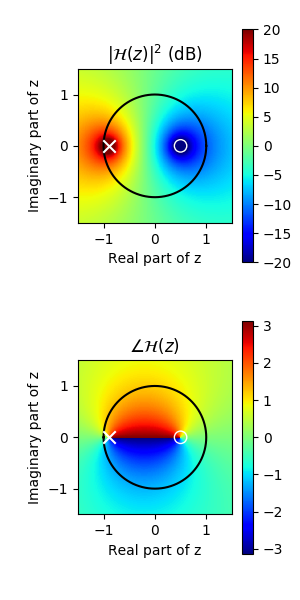
\includegraphics[width=\textwidth]{code/026_iir/z_mag_angle_iir.png}
\caption{The magnitude of the system function given in Equation \ref{eq:example_iir_system_hpf}. The white cross indicates the pole at $z=-0.9$ and the white circle indicates the zero at $z=0.5$. The black circle indicates the unit circle.}
\label{fig:pz_diag}
\end{marginfigure}
By comparing the system function in Equation \ref{eq:coeffs_read} with
Equations \ref{eq:iir_def} and \ref{eq:iir_system_gen}, we can see
that the system is described using the following difference equation:
\begin{marginfigure}
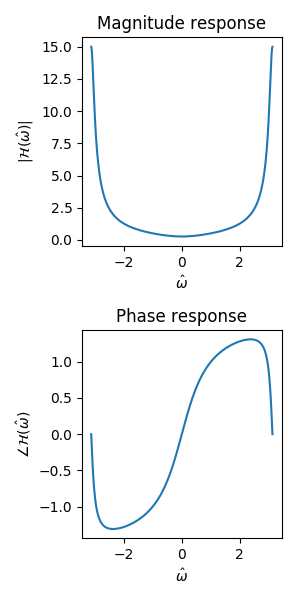
\includegraphics[width=\textwidth]{code/026_iir/z_mag_angle_iir2.png}
\caption{The magnitude and frequency response of the system given in Equation \ref{eq:example_iir_system_hpf}. This filter is a high-pass filter.}
\label{fig:pz_diag2}
\end{marginfigure}
\begin{equation}
y[n] = -0.9 y[n-1] +x[n] - 0.5x[n-1]
\end{equation}

The impulse response is a polynomial fraction. We can multiply this by
$z/z$ to obtain:
\begin{equation}
\Hez = \frac{z-0.5}{z+0.9} = \frac{P(z)}{Q(z)}.
\label{eq:example_iir_system_hpf}
\end{equation}
The numerator polynomial $P(z)$ has a zero at $z=0.5$, and the
denominator polynomial $Q(z)$ has a zero at $z=-0.9$. This means that
$\mathcal{H}(0.5)=0$ and $\mathcal{H}(-0.9)\rightarrow \infty$. The
zeros of $P(z)$ and $Q(z)$ have the opposite effect on the signal.

Zeros of the denominator polynomial $Q(z)$ are called \emph{poles} of
the system function. They indicate signals
$\mathcal{T}\{z^{n}\} \rightarrow \infty$ for which the output of the
system grows exponentially.


Figure \ref{fig:pz_diag} shows the magnitude of the system function
$|\Hez|$ on the complex plane. The pole at $z=-0.9$ is indicated with
a white cross, and the zero at $z=0.5$ is indicated with a white
circle. We can see the implication of the zeros and the poles of the
system function. The system function has a large magnitude near the
poles and low values in the region near the zeros.

A plot like the one shown in Figure \ref{fig:pz_diag} is known as a
\emph{\index{pole-zero diagram}{pole-zero diagram}}. Typically such a diagram only depicts the locations
of the poles and zeros with crosses and circles. These diagrams are
useful for analyzing the properties of discrete-time LTI systems.

We can obtain the frequency response of the system by evaluating
$\mathcal{H}(z)$ on the unit circle:
\begin{equation}
\mathcal{H}(\hat{\omega}) = \frac{e^{i\hat{\omega}}-0.5}{e^{i\hat{\omega}}+0.9}
\end{equation}
This is shown in Figure \ref{fig:pz_diag2}. This filter is a high-pass
filter.




\if 0
\subsection{Example: step response of 1st order IIR-filter}

In order to get an idea of stability, let us consider a first order IIR filter, which is defined as:
\begin{equation}
y[n] = a y[n-1] + b x[n].
\end{equation}
This has an impulse response:
\begin{equation}
h[n] = b a^n u[n].
\end{equation}
If we now use the unit step function as input to this system $x[n]=u[n]$, we obtain the following output:
\begin{align}
y[n] &= \sum_{k=-\infty}^{\infty} h[k]x[n-k]  \\
     &= \sum_{k=-\infty}^{\infty} b a^k u[k]u[n-k]
\end{align}
Because 
\begin{equation}
u[k]u[n-k] = \left\{\begin{array}{cc}
1 & 0 \le k \le n\\
0 & \mathrm{otherwise}
\end{array}
\right.
\end{equation}
we get finite bounds for the sum:
\begin{align}
y[n] &= b \sum_{k=0}^{n} a^k.
\end{align}
This again is a geometric series. The output of the system fed with a unit impulse is thus:
\begin{align}
y[n] &= b\frac{1-a^{n+1}}{1-a}.
\end{align}
It is possible to identify two distinct cases for asymptotic behavior:
\begin{enumerate}
\item $|a|>1$ $\Rightarrow$ $\lim_{n\rightarrow \infty} |y[n]| = \infty$. The system output magnitude increases exponentially without bound.
\item $|a|<1$ $\Rightarrow$ $\lim_{n\rightarrow \infty}y[n]=\frac{b}{1-a}$. The output is finite. 
\end{enumerate}
Hence: if $|a|<1$, then the filter output is finite. If $|a|>1$, the magnitude of the output grows exponentially. 
\subsection{Example: poles and zeros for 1st order IIR-filter}
The first order IIR filter has the following system function:
\begin{align}
\Hez &= \left.\frac{b_0 + b_1 z^{-1}}{1-a z^{-1}} \right| \cdot \frac{z}{z} \\
     &= \frac{b_0 z + b_1}{z-a}
\end{align}
The system function has
\begin{enumerate}
\item a zero ($\Hez = 0)$ at $z=-\frac{b_1}{b_0}$,
\item and a pole ($\Hez \rightarrow \infty)$ for $z=a$.
\end{enumerate}
The magnitude and phase of the system function are shown below in the case where $a=-0.9$, $b_1=1$ and $b_0=-2$ the zero is located at $z = \frac{1}{2}$ and the pole is located at $z=-0.9$:
\begin{center}
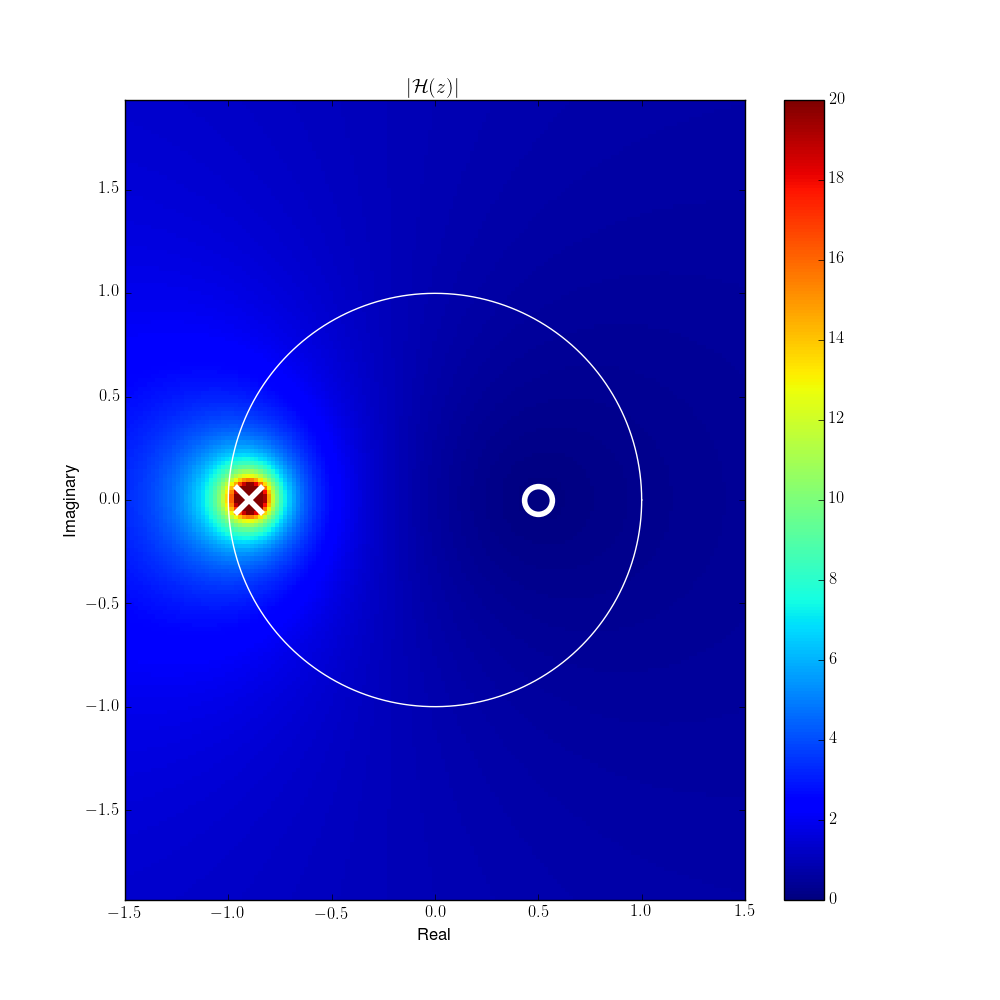
\includegraphics[width=0.45\textwidth]{ch19/figures/zcol_iir0.png}
\includegraphics[width=0.45\textwidth]{ch19/figures/zcol_iir0p.png}
\includegrpahics[width=0.6\textwidth]{ch19/figures/iir_stable.png}
\end{center}
This first order system has the following impulse response:
\begin{equation}
h[n] = b_0 a^n u[n] + b_1 a^{n-1} u[n-1].
\end{equation}
From this we can see that:
\begin{enumerate}
\item If $|a|<1$, the impulse response will die out as $n\rightarrow \infty$. The output of the filter has a \emph{stable} output if the pole $z=a$ is inside the unit circle.
\item If $|a|\ge 1$, the impulse response will not die out as $n\rightarrow \infty$. The output of the filter is \emph{unstable}, and the pole is at the unit circle or outside it.
\end{enumerate}
\fi

\section{Stability for an arbitrary IIR system}

Because of the feedback terms in IIR systems, these systems are not
necessarily stable. Instability means that the output of the system
for some inputs can become indeterminate. This is one of the main
drawbacks of IIR systems.

\index{Bounded Input Bounded Output}{Bounded Input Bounded Output} (BIBO) \index{stability}{stability} is used to determine the
stability of an IIR system. BIBO stability implies that for a bounded
input:
\begin{equation}
|x[n]| \le M_x < \infty.
\end{equation}
the output is also bounded:
\begin{equation}
|y[n]| \le M_y < \infty.
\end{equation}
The output of a filter is a convolution sum of the input signal $x[n]$
convolved with the impulse response $h[n]$ of the system. In the case
of an LTI system, the magnitude of the output is:
\begin{equation}
|y[n]| = \left| \sum_{k=-\infty}^{\infty} h[k] x[n-k]\right|
\end{equation}
Using the triangle inequality ($c = a+b$ $\Rightarrow$ $|c|\le |a|+|b|$), we can obtain the following bounds:
\begin{equation}
\left|\sum_{k=-\infty}^{\infty} h[k]x[n-k]\right| \le \sum_{k=-\infty}^{\infty}|h[k]|\underbrace{|x[n-k]|}_{\le M_x} \le M_x \sum_{k=-\infty}^{\infty}|h[k]|.
\end{equation}
Thus, a sufficient condition for bounded output $|y[n]| \le M_y < \infty$ given a bounded input $|x[n]|\le M_x < \infty$ is that the impulse response $h[n]$ is bounded to some finite value $M_h$:
\begin{equation}
\boxed{
\sum_{k=-\infty}^{\infty} |h[k]| \le M_h < \infty.
}
\end{equation}

\subsection{Example: Stability of a first order IIR system}

A first order system has the following system function:
\begin{equation}
\Hez = \frac{b}{1-a z^{-1}}
\end{equation}
When is this system stable?

The impulse response of this system is:
\begin{equation}
h[n] = b a^n u[n].
\label{eq:iir_stab_1}
\end{equation}
Using the BIBO stability criterion, the output of this system is
stable if:
\begin{align}
\sum_{k=-\infty}^{\infty} |h[k]| \le M_h < \infty.
\end{align}
Using Equation \ref{eq:iir_stab_1}, we obtain:
\begin{align}
\sum_{k=-N}^{N} |h[k]| &= \sum_{k=-N}^{N} |b a^k u[k]|\\
&= |b| \sum_{k=0}^{N}|a|^k
\end{align}
If $|a|\ge 1$, then
\begin{align}
\sum_{k=-\infty}^{\infty} |h[k]| &= \lim_{N\rightarrow \infty} |b| \sum_{k=0}^{N}|a|^k \rightarrow \infty
\end{align}
The system is BIBO unstable if $|a| \ge 1$.

We can use the geometric series solution formula for the case $|a| < 1$:
\begin{align}
|b| \sum_{k=0}^{N}|a|^k = |b| \frac{1-|a|^{N+1}}{1-|a|}.
\end{align}
A limit of the infinite sum is thus a limit of the finite sum:
\begin{equation}
\sum_{k=-\infty}^{\infty} |h[k]| = \lim_{N\rightarrow \infty} |b|\frac{1-|a|^{N+1}}{1-|a|}.
\end{equation}
When $|a|<1$, we get:
\begin{equation}
\sum_{k=-\infty}^{\infty} |h[k]| = \frac{|b|}{1-|a|} < \infty.
\end{equation}
The system is BIBO stable when $|a|<1$.

\begin{marginfigure}[-5cm]
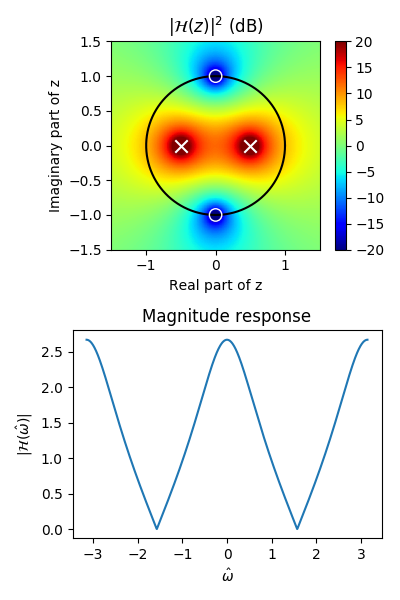
\includegraphics[width=\textwidth]{code/026_iir/ex1.png}
\caption{A band-stop filter.}
\label{fig:pzex1}
\end{marginfigure}
\begin{marginfigure}[-5cm]
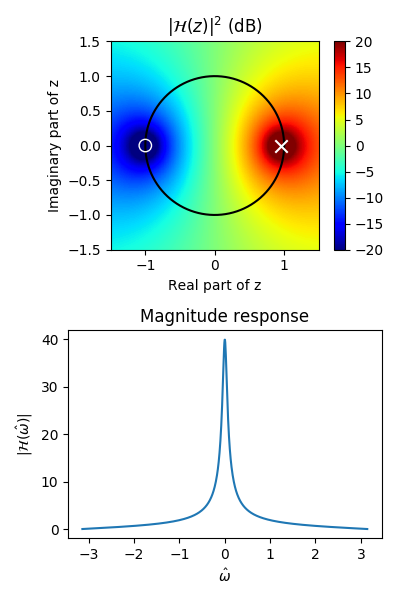
\includegraphics[width=\textwidth]{code/026_iir/ex4.png}
\caption{A low-pass filter.}
\label{fig:pzex2}
\end{marginfigure}

\section{Poles and zeros}

An arbitrary order IIR system has a system function, which is a polynomial fraction:
\begin{equation}
\Hez = \frac{\sum_{k=0}^{M}b_{k}z^{-k}}{1-\sum_{\ell=1}^{N}a_{\ell} z^{-\ell}} = \frac{P(z)}{Q(z)}.
\end{equation}
The fundamental theorem of algebra says that because the numerator
polynomial $P(z)$ is an $M$th order polynomial, it has $M$ values of
$z=\alpha_k$ for which $P(\alpha_k)=0$. 

Similarly, the denominator polynomial $Q(z)$ is an $N$th order
polynomial, which has $N$ roots $Q(\beta_{\ell})=0$. 

We will assume that all the zeros of the numerator and denominator
are distinct: $\alpha_{k} \ne \alpha_{\ell}$,
$\alpha_{k} \ne \beta_{\ell}$, and $\beta_{k} \ne \beta_{\ell}$ for
all $k\ne \ell$. We'll also assume that $M>0$, that there is at least
one zero of the numerator polynomial.

We can then express the system function of an IIR filter in the
following form:
\begin{equation}
\Hez = \frac{\prod_{k=1}^{M}(z-\alpha_{k})}{\prod_{\ell=1}^{N}(z-\beta_{\ell} )} =  \frac{\prod_{k=1}^{M}(1-\alpha_{k}z^{-1})}{\prod_{\ell=1}^{N}(1-\beta_{\ell} z^{-1})} = \frac{P(z)}{Q(z)}
\end{equation}
The terms $\beta_{\ell}$ are the \emph{\index{poles}{poles}} of the
system function. They indicate regions of the complex plane where the
system function magnitude approaches infinity
$\mathcal{H}(\beta_{\ell})\rightarrow \infty$.

The terms $\alpha_{k}$ are the \emph{\index{zeros}{zeros}} of the
system function. They indicate regions of the complex plane where the
system function magnitude becomes zero valued $\mathcal{H}(\alpha_{k}) = 0$.
\begin{marginfigure}[-5cm]
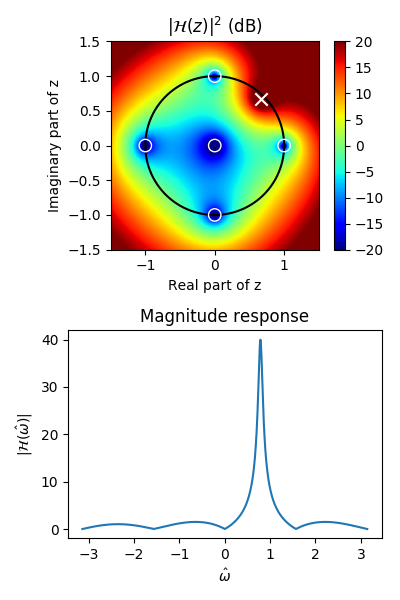
\includegraphics[width=\textwidth]{code/026_iir/ex7.png}
\caption{A band-pass filter that passes through positive frequencies. The resulting signal will be complex valued, even if a real valued signal is fed into the system.}
\label{fig:pzex3}
\end{marginfigure}

\subsection{Example: Pole-zero diagrams}

By knowing the poles and zeros of the system function, it is possible
to analytically say quite a lot about the behavior of the
filter. Figures \ref{fig:pzex1}, \ref{fig:pzex2}, \ref{fig:pzex3}
and \ref{fig:pzex4} show some examples of \index{pole-zero
diagrams}{pole-zero diagrams} and the magnitude responses associated
with these filters. It is possible to tell from the positions of the
poles and zeros what type of magnitude response the filter has.

\if 0
\begin{figure}
\begin{center}
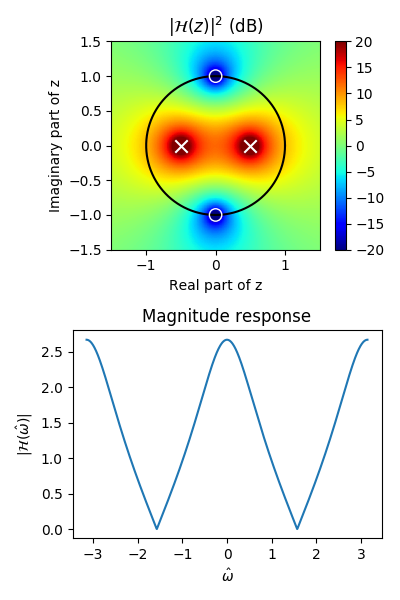
\includegraphics[width=0.49\textwidth]{code/026_iir/ex1.png}
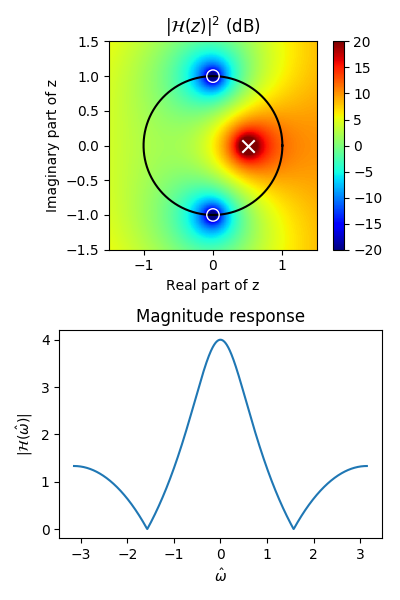
\includegraphics[width=0.49\textwidth]{code/026_iir/ex2.png}
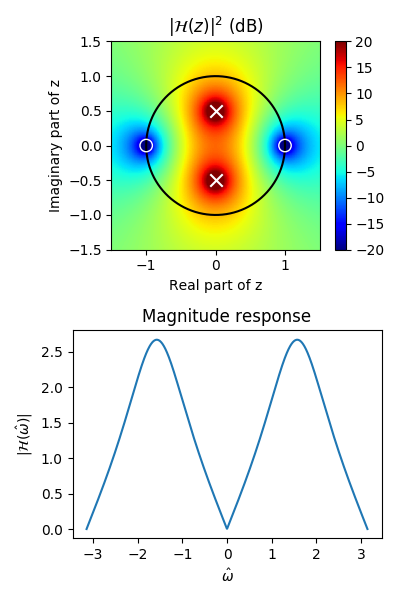
\includegraphics[width=0.49\textwidth]{code/026_iir/ex3.png}
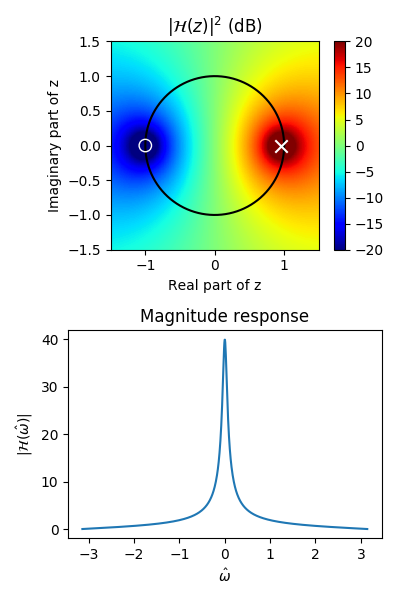
\includegraphics[width=0.49\textwidth]{code/026_iir/ex4.png}
\end{center}
\caption{Examples of pole-zero diagrams together and the magnitude responses of the filters corresponding to each system function. The locations of the poles are indicated with white crosses, and the locations of the zeros are indicated with white circles. Top left: band-stop filter, which rejects frequency $\hat{\omega}=\pm\pi/2$. Top right: low-pass filter. Bottom left: band-pass filter, which passes frequency $\hat{\omega}=\pm \pi/2$. Bottom right: low-pass filter.}
\label{fig:pz_examples}
\end{figure}

\begin{figure}
\begin{center}
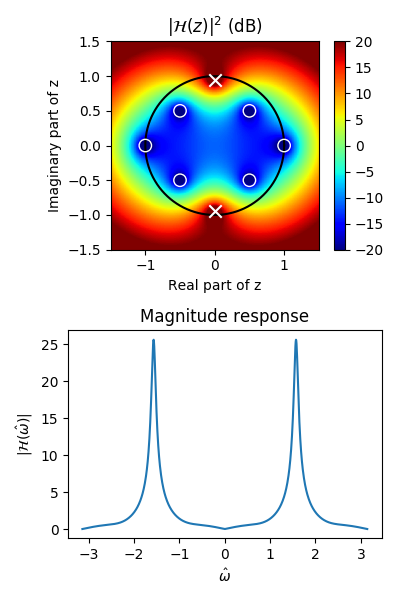
\includegraphics[width=0.49\textwidth]{code/026_iir/ex5.png}
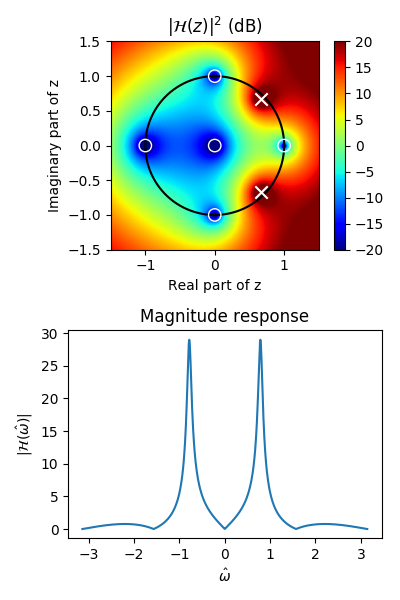
\includegraphics[width=0.49\textwidth]{code/026_iir/ex6.png}
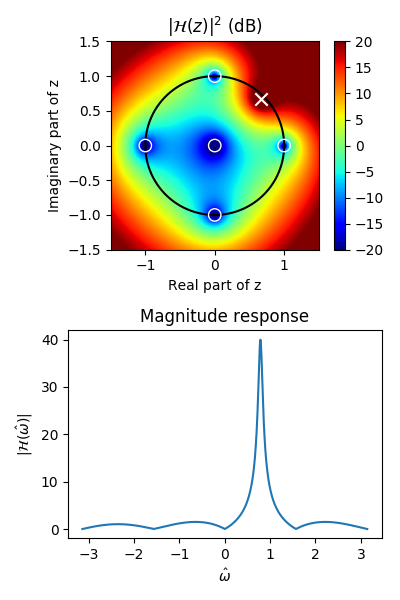
\includegraphics[width=0.49\textwidth]{code/026_iir/ex7.png}
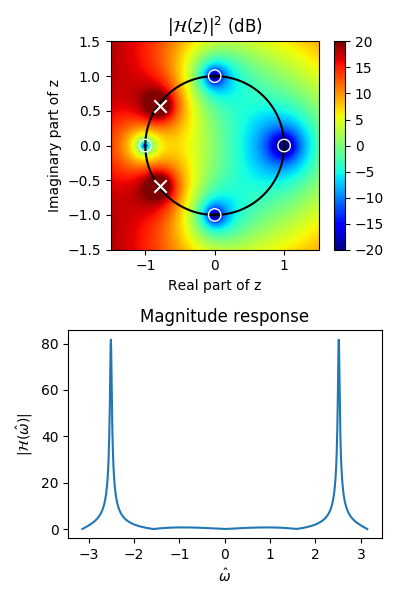
\includegraphics[width=0.49\textwidth]{code/026_iir/ex8.png}
\end{center}
\caption{Examples of pole-zero diagrams together and the magnitude responses of the filters corresponding to each system function. The locations of the poles are indicated with white crosses, and the locations of the zeros are indicated with white circles. Top left: band-stop filter, which rejects frequency $\hat{\omega}=\pm\pi/2$. Top right: low-pass filter. Bottom left: band-pass filter, which passes frequency $\hat{\omega}=\pm \pi/2$. Bottom right: low-pass filter.}
\label{fig:pz_examples2}
\end{figure}
\fi

\section{Partial fraction decomposition}

\begin{marginfigure}
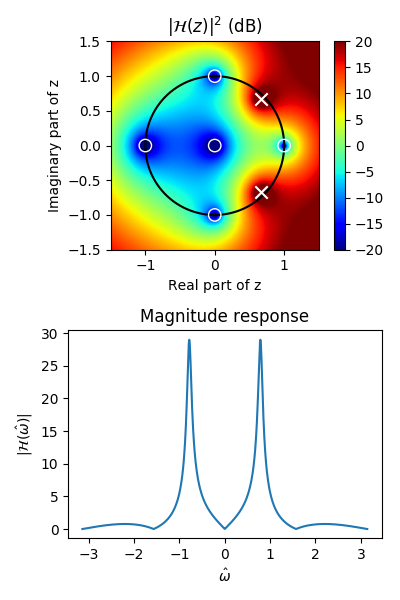
\includegraphics[width=\textwidth]{code/026_iir/ex6.png}
\caption{A band-pass filter}
\label{fig:pzex4}
\end{marginfigure}

Using \emph{\index{partial fraction decomposition}{partial fraction
decomposition}}, we can refactor the system function of an IIR filter
in such a way that we can easily calculate an inverse $z$-transform of
the system function using the elementary first order IIR filter
$z$-transform pair that we covered earlier. I won't provide the general
formulation here. Instead, I'll demonstrate this with an example,
which can be generalized for higher order IIR systems.

\subsection{Example: Partial fraction decomposition $N=2$ and $M=2$}

Consider the case where the system function of an IIR filter is defined as:
\begin{equation}
\Hez= \frac{b_0 + b_1 z^{-1} + b_2 z^{-2}}{(1-\beta_1 z^{-1})(1-\beta_2 z^{-1})}.
\label{eq:original_pfe}
\end{equation}
What is the impulse response of this system? Is this filter BIBO
stable?

Note that the denominator of Equation \ref{eq:original_pfe} is already
expressed in a form where $\beta_1$ and $\beta_2$ correspond to the poles
of the system function.

The order of the numerator and denominator is $N=M=2$. In this case,
the partial fraction decomposition results in the following form:
\begin{equation}
\Hez = \frac{A}{1-\beta_1 z^{-1}} + \frac{B}{1-\beta_2 z^{-1}} + C,
\end{equation}
where $A$, $B$, and $C$ are coefficients that need to be determined. 

We can determine what these coefficients are:
\begin{align}
\Hez &= \frac{A(1-\beta_2 z^{-1})+B(1-\beta_1 z^{-1})+C(1-\beta_1 z^{-1})(1-\beta_2 z^{-1})}{(1-\beta_1 z^{-1})(1-\beta_2 z^{-1})} \\
     &= \frac{ (A+B+C) + (-A\beta_2 -B \beta_1 - C(\beta_1+\beta_2))z^{-1} + (C\beta_1 \beta_2)z^{-2}}{(1-\beta_1 z^{-1})(1-\beta_2 z^{-1})}\label{eq:pfe_fac}.
\end{align}
By comparing Equation \ref{eq:original_pfe} with
Equation \ref{eq:pfe_fac}, we get a set of linear equations, which can
be used to solve for coefficients $A$, $B$, and $C$:
\begin{equation}
\left\{ \begin{array}{cc}
A+B+C &= b_0 \\
-A\beta_2-B\beta_1-C(\beta_1+\beta_2) &= b_1 \\
C\beta_1\beta_2 &= b_2 \\
\end{array}
\right.
\end{equation}
The inverse $z$-transform can then be done using known $z$-transform pairs:
\begin{equation}
a\delta[n-n_0] \xleftrightarrow{\mathcal{Z}} a z^{-n_0}
\end{equation}
and
\begin{equation}
b a^n u[n] \xleftrightarrow{\mathcal{Z}} \frac{b}{1-az^{-1}}.
\end{equation}
The time-domain impulse response $h[n]$ is therefore:
\begin{equation}
h[n] = A \beta_1^n u[n] + B \beta_2^n u[n] + C\delta[n].
\end{equation}

In order to address the question of filter stability, we can now apply
our previous BIBO stability result for first order IIR filter impulse
response. The filter is stable as long as $|\beta_1|<1$ and
$|\beta_2|<1$. In other words, the filter is stable if all the
poles of the system function are inside the unit circle.

\section{IIR filtering with Scipy}

It is possible to implement an IIR filter using Scipy. There is a
function \verb|scipy.signal.lfilter|, which implements an IIR
filtering operation.

The function \verb|lfilter| expects the filter coefficients to be specified in the following format:
\begin{equation}
\Hez = \frac{{\color{red}b_0} + {\color{red}b_1} z^{-1} + {\color{red}b_2} z^{-2} + \cdots + {\color{red}b_N} z^{-N}}{{\color{blue}1} + {\color{blue}a_1} z^{-1} + {\color{blue}a_2} z^{-2} + \cdots + {\color{blue}a_M} z^{-M}}
\end{equation}
The example filter that is defined in Equation \ref{eq:coeffs_read} is as follows:
\begin{align}
\Hez &= \frac{1-0.5z^{-1}}{1+0.9 z^{-1}}
\label{eq:sys_ex}
\end{align}
In Python, we would form two vectors: {\color{red}\verb|b=[1,-0.5]|}
and {\color{blue}\verb|a=[1,0.9]|} and pass these to \verb|lfilter(b,a,signal)| to
IIR filter a vector \verb|signal|.


The Python code in Listing \ref{lst:simple_hpf} demonstrates
implementing the IIR filter that has the system function defined in
Equation \ref{eq:sys_ex}. It filters a Gaussian random noise signal,
which has a flat power spectrum. How the filter modifies this spectrum
allows us to inspect what the filter does to the signal. The code also
has a simple routine that demonstrates how the same IIR filter could be
naively implemented without resorting to a library function.


\begin{marginfigure}
\begin{center}
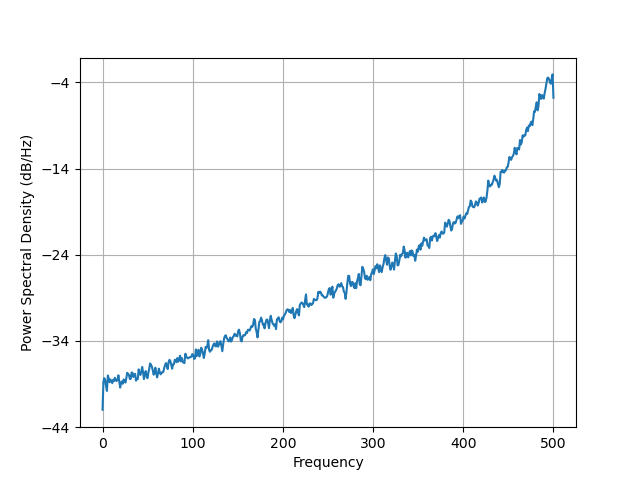
\includegraphics[width=\textwidth]{code/026_iir/ex_psd_hpf.png}
\end{center}
\caption{The power spectrum estimate of the filtered white noise signal using the simple high-pass filter specified in Equation \ref{eq:sys_ex}. Compare this with the analytical magnitude response shown in Figure \ref{fig:pz_diag2}}
\end{marginfigure}

\lstinputlisting[language=Python,caption={\texttt{026\_iir/simple\_hpf.py}},label=lst:simple_hpf]{code/026_iir/simple_hpf.py}

\section{IIR filter design with Scipy}

Scipy includes an IIR filter design
routines \verb|scipy.signal.iirfilter|
and \verb|scipy.signal.iirdesign|. These functions can be used to
design \index{bandpass}{bandpass}, \index{lowpass}{lowpass}, \index{highpass}{highpass},
and \index{bandstop}{bandstop} filters that meet design
specifications.

Scipy functions \verb|scipy.signal.lfilter|
and \verb|scipy.signal.sosfilt| can be used to filter signals using an
IIR filter.

\begin{marginfigure}
\begin{center}
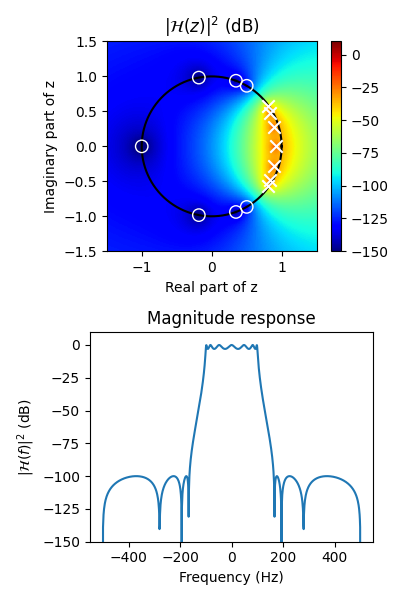
\includegraphics[width=\textwidth]{code/026_iir/ex_design_lpf.png}
\end{center}
\caption{The pole-zero diagram and magnitude response of the designed IIR low-pass filter. The bandwidth is specified to be 100 Hz, with the stop-band starting at 200 Hz. Spectral components of the signal in the stop-band are attenuated by at least 100 dB.}
\label{fig:iir_lpf_ex_sf}
\end{marginfigure}

The Python code in Listing \ref{lst:iir_design} shows an example of
designing an IIR low-pass filter. The filter cutoff is set to be 100
Hz and the filter band-stop is set to be 200 Hz. The minimum
attenuation for signals with frequencies higher than 200 Hz is set to
be 100 dB.

I then generate a Gaussian random signal and filter this signal using
the low-pass filter that was designed. A Gaussian random noise has a
flat power spectrum, which allows us to investigate how the filter
shapes this spectrum.

Finally, I use the \verb|matplotlib.pyplot.psd| function to estimate
the power spectrum of the filtered signal.


\begin{marginfigure}
\begin{center}
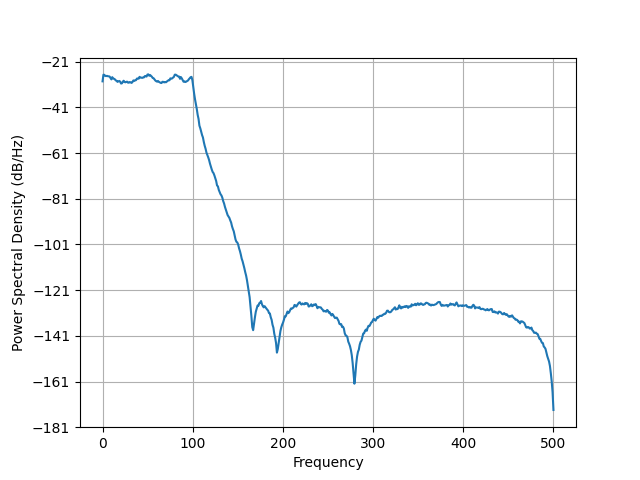
\includegraphics[width=\textwidth]{code/026_iir/ex_psd_lpf.png}
\end{center}
\caption{A power spectrum estimate of the filtered signal. The spectrum looks nearly identical to the analytic magnitude response of the filter shown in Figure \ref{fig:iir_lpf_ex_sf}.}
\end{marginfigure}

\lstinputlisting[language=Python,caption={\texttt{026\_iir/iir\_design.py}},label=lst:iir_design]{code/026_iir/iir_design.py}







